\documentclass[xcolor=dvipsnames, notes=hide]{beamer}
%\documentclass[xcolor=dvipsnames, notes=only]{beamer}
%\documentclass[xcolor=dvipsnames]{beamer}
%\setbeameroption{show only notes}
%\usepackage{pgfpages}
%\setbeamertemplate{note page}[plain]
%\setbeameroption{show notes on second screen=right}

\usepackage[english]{babel}
\usepackage[utf8]{inputenc}
\usepackage[T1]{fontenc} % Ligaturen, richtige Umlaute im PDF

\newcommand{\IR}{\mathbb{R}}
\newcommand{\backupbegin}{
	\newcounter{finalframe}
	\setcounter{finalframe}{\value{framenumber}}
}
\newcommand{\backupend}{
	\setcounter{framenumber}{\value{finalframe}}
}

\usepackage[absolute,overlay]{textpos} % textblock for figure placement

\usepackage{tabularx, booktabs}
\usepackage{amsmath}
\usepackage{blkarray, bigstrut}
\usepackage{xparse}

\usepackage[normalem]{ulem} % for \sout{}
\usepackage[ruled]{algorithm}
\usepackage{algpseudocode} 
\makeatletter
\def\BState{\State\hskip-\ALG@thistlm}
\algdef{SE}[DOWHILE]{Do}{doWhile}{\algorithmicdo}[1]{\algorithmicwhile\ #1}
\makeatother

\beamertemplatenavigationsymbolsempty
%\selectlanguage{english}
\usepackage{biblatex}
\bibliography{Bibliography}

\usepackage{bbm} % For mathbb{1}
\usepackage{csquotes}
\usepackage{colordvi}
\usepackage{xcolor}
%\usepackage{foiltex}

%\usepackage{enumitem}

\usepackage{tikz}
\usetikzlibrary{positioning}
\graphicspath{{/images/}}


\usetheme{CambridgeUS}
% Other valid themes
%   Antibes, Bergen, Berkeley, Berlin, Copenhagen
%   Darmstadt, Dresden, Frankfurt, Goettingen, Hannover
%   Ilmenau, JuanLesPins, Luebeck, Madrid, Malmoe
%   Marburg, Montpellier, PaloAlto, Pittsburgh, Rochester
%   Singapore, Szeged, Warsaw, boxes, default

%\usecolortheme{beetle}
%\usecolortheme{dolphin}
% Other valid color schemes
%    albatross, beaver, beetle, crane, dolphin
%    dove, fly, lily, orchid, rose, seagull
%    seahorse, whale and the one and only wolverine

%%%%%%%%%%%%%%%%%%%%%%%%%%%%%%%%
%%%%% PyCharm Color Scheme %%%%%
%%%%%%%%%%%%%%%%%%%%%%%%%%%%%%%%

%%% COLOR DEFINITIONS
\definecolor{uniBonnBlueDark}{HTML}{004F9F}
\definecolor{uniBonnYellow}{HTML}{F4B400} % lighter shades: FFDE85, FFD35C

\definecolor{pyCharmBgMain}{HTML}{2B2B2B} % RGB: 43, 43, 43

\definecolor{titleCardBg}{HTML}{CFCFEF} % former: F6511D (orange), CFCFEF (light purple) 

\definecolor{pyCharmBgSecond}{HTML}{313335}
\definecolor{pyCharmFgSecond}{HTML}{9F9FAF} % RGB: 159, 159, 175

\definecolor{pyCharmGreen}{HTML}{499C54} % RGB: 73, 156, 84

%%% Original PyCharmColors:
%\definecolor{pyCharmBgMain}{HTML}{2B2B2B}
%\definecolor{pyCharmFgMain}{HTML}{88B1AC}
%\definecolor{pyCharmBgSecond}{HTML}{313335}
%\definecolor{pyCharmFgSecond}{HTML}{5D5F53}
%\definecolor{pyCharmGreen}{HTML}{499C54}

%%% COLOR SETTINGS
\setbeamercolor{background canvas}{fg=pyCharmFgSecond, bg=pyCharmBgMain}
\setbeamercolor{background}{fg=pyCharmFgSecond, bg=pyCharmBgMain}

\setbeamercolor{normal text}{fg=pyCharmFgSecond,bg=pyCharmFgSecond}
\setbeamercolor{alerted text}{fg=red}

\setbeamercolor{palette primary}{fg=pyCharmFgSecond, bg=pyCharmBgSecond}
\setbeamercolor{palette secondary}{fg=pyCharmFgSecond, bg=pyCharmBgSecond}
\setbeamercolor{palette tertiary}{fg=white, bg=uniBonnBlueDark}

\setbeamercolor{frametitle}{bg=pyCharmBgSecond, fg=pyCharmFgSecond}
\setbeamercolor{title}{fg=uniBonnBlueDark, bg=titleCardBg}

\setbeamercolor{local structure}{fg=pyCharmGreen} % light green
\setbeamercolor{subsection in toc}{bg=pyCharmBgMain, fg=pyCharmGreen}
\setbeamercolor{section in toc}{bg=pyCharmBgMain, fg=pyCharmGreen}

% For figure captions
\setbeamercolor{caption}{fg=pyCharmFgSecond}
\setbeamercolor{caption name}{fg=pyCharmGreen}

\setbeamertemplate{itemize item}{fg=pyCharmGreen$\blacksquare$}
\setbeamertemplate{itemize subitem}{\color{499C54}$\blacksquare$}
\setbeamertemplate{itemize items}[default]
\setbeamertemplate{enumerate items}[default]

\setbeamertemplate{section in toc}{%
	{\color{pyCharmGreen} \inserttocsectionnumber.}\color{pyCharmFgSecond}~\inserttocsection}
\setbeamertemplate{subsection in toc}{%
	\hspace{1.2em}{\color{pyCharmGreen}\rule[0.3ex]{3pt}{3pt}} ~\inserttocsubsection\par}

\renewcommand{\textbf}[1]{{\bfseries\color{pyCharmGreen}#1}}

\setbeamercolor*{palette tertiary}{bg=uniBonnBlueDark}

%%% LOGO PLACEMENT
\addtobeamertemplate{frametitle}{}{%
	\begin{tikzpicture}[remember picture,overlay]
	\node[anchor=north east,yshift=-3pt] at (current page.north east) {
		
\includegraphics[height=0.8cm]{images/UNI_Bonn_Logo_Standard_RZ_XL.png}
		
\includegraphics[height=0.8cm]{images/AG_logo_hp_70x70.png}
	};
	\end{tikzpicture}}
%\addtobeamertemplate{frametitle}{}{%
%	\begin{tikzpicture}[remember picture,overlay]
%	\node[anchor=north east,yshift=-9pt] at (current page.north east) {
%		
\includegraphics[height=0.8cm]{images/UNI_Bonn_Logo_Standard_RZ_XL.png}
%		
\includegraphics[height=0.8cm]{images/AG_logo_hp_70x70.png}
%	};
%	\end{tikzpicture}}
% !Tex spellceck = en_US

\title[MA Seminar Talk - Progress]{Master Thesis Seminar Talk}
\subtitle{Progress Upade}
\author[F. Beaumont]{Fabrice Beaumont}
\institute[]{Lab Development and Application of Data Mining and Learning Systems: \\ Machine Learning and Data Mining \\ \vspace{0.5 cm} Supervisor: \textbf{Dr. Pascal Welke}\\
}
\date{19. January 2022}
\begin{document}


\begin{frame}
	\titlepage
\end{frame}

% 2
\begin{frame}
\frametitle{Research question - overview}
\begin{figure}[H]
	\centering
	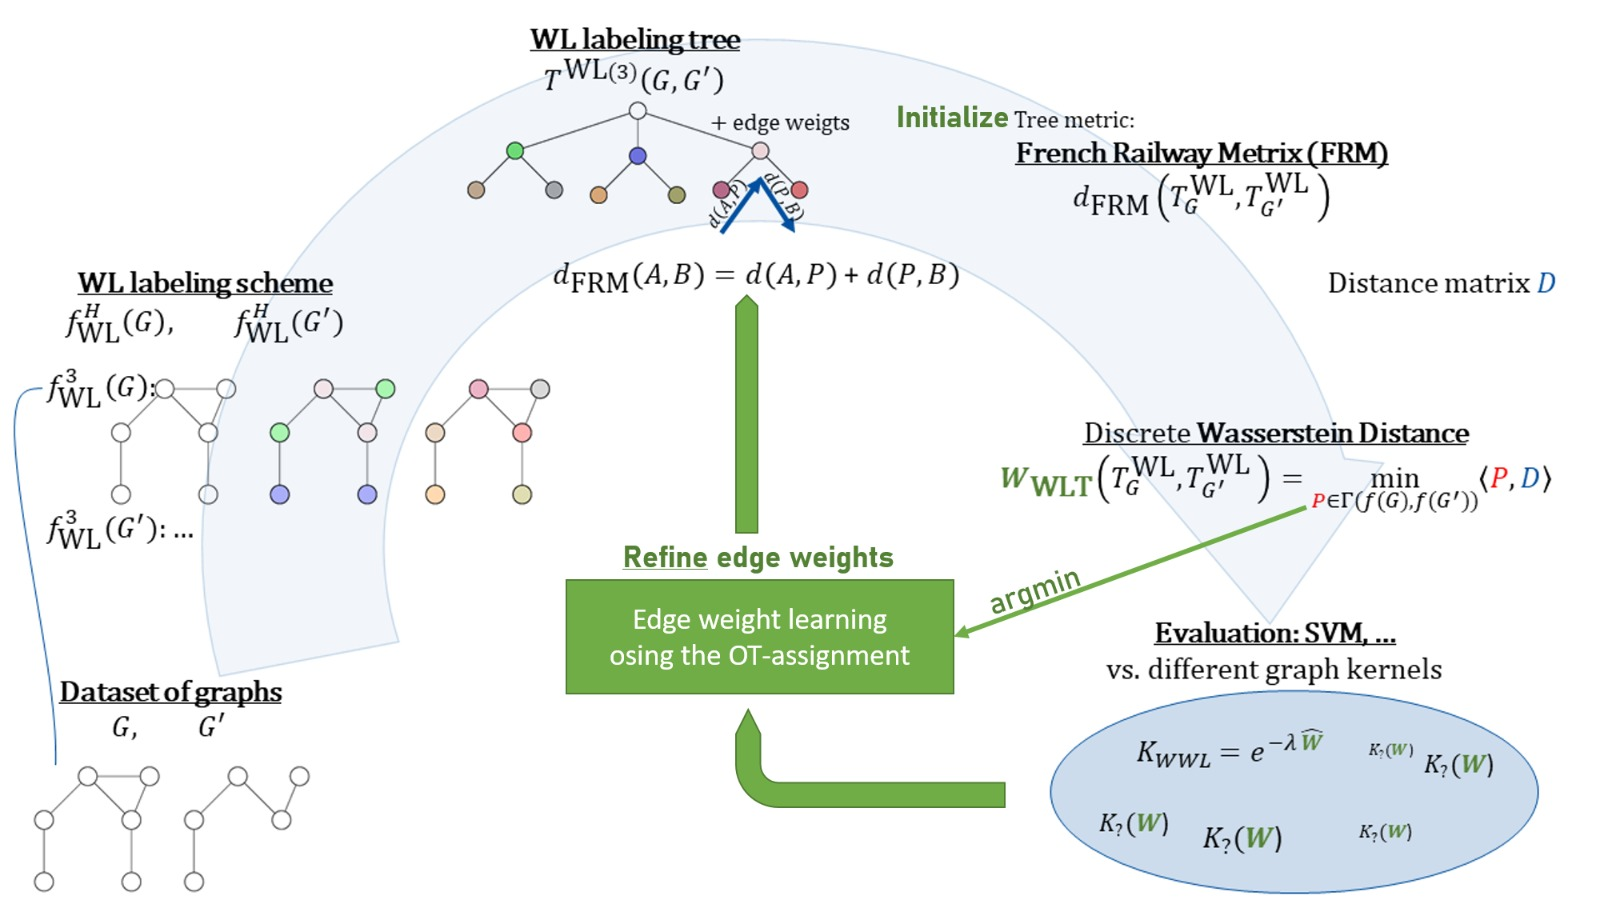
\includegraphics[width=1.0\linewidth]{images/MasterThesisOverview}
	\label{fig:MasterThesisOverview}
\end{figure}
\end{frame}

% 3
\begin{frame}
\frametitle{Research question - draft}
	\begin{center}
		\textbf{Does the (chosen) iterative weight adjustment\newline\\
		lead to a significant increase in the\newline\\
		expressiveness of the resulting kernel?}
	\end{center}
\end{frame}

% 4 
\begin{frame}
\frametitle{Method overview} \vspace{-1cm}
	\begin{enumerate}
		\item \begin{tabbing}
			Given: \=Graph database $\mathcal{D}=\{ (V_i, E_i, \ell^V_i) \}_{i\in[N]}$\\
			\>Distance $d$ on $\bigcup_{i\in[N]}\text{Range}(\ell^V_i)$\ \ \=for the FRM\\
			\>Ground distance $d_0$\>for the Wass.Dist. $W_{\text{WLT}}$
		\end{tabbing}
		\item Compute $t$ iterations of Weisfeiler Lehman (WL) labels on $\mathcal{D}$
		\item Construct the WL labeling tree (WLLT) [WL labeling hierarchy]
		\item Define edge weights on the WLLT - using a FRM (and $d$)		
		\item Define an \underline{initial} distance between graphs - using $W_{\text{WLT}}$ (and $d_0$)
	\end{enumerate}
	\hfill\newline
	\begin{itemize}		
		\item[] \hfill\newline
		\item[] \hfill\newline
	\end{itemize}
\end{frame}

% 4 
\begin{frame}
\frametitle{Method overview} \vspace{-1cm}
\begin{enumerate}
	\item \begin{tabbing}
		Given: \=Graph database $\mathcal{D}=\{ (V_i, E_i, \ell^V_i) \}_{i\in[N]}$\\
		\>Distance $d$ on $\bigcup_{i\in[N]}\text{Range}(\ell^V_i)$\ \ \=for the FRM\\
		\>Ground distance $d_0$\>for the Wass.Dist. $W_{\text{WLT}}$
	\end{tabbing}
	\item Compute $t$ iterations of Weisfeiler Lehman (WL) labels on $\mathcal{D}$
	\item Construct the WL labeling tree (WLLT) [WL labeling hierarchy]
	\item Define edge weights on the WLLT - using a FRM (and $d$)		
	\item Define an \underline{initial} distance between graphs - using $W_{\text{WLT}}$ (and $d_0$)
\end{enumerate}
\textbf{Loop:}
\begin{itemize}		
	\item Use the distances to define a WWL-kernel and classify the database using an SVM
	\item Use the mapping chosen by $W_{\text{WLT}}$ to identify crucial edge weights. \textbf{Refine the edge weights}, given the desired closeness of the graphs.
\end{itemize}
\end{frame}

% 5
\begin{frame}
\frametitle{Current progress}
	Programming:
	\begin{itemize}
		\item Construction of the WL-labeling tree (WLLT) \newline
		\item Several distance metrics for this WLLT \newline
		\item Construction of the WL-label set representation of the graphs \newline
		\item Construction of a distance matrix/kernel on the dataset\newline
	\end{itemize}	
	Still in progress: Several optimizations w.r.t to these implementations.
\end{frame}

% 6
\begin{frame}
\frametitle{Next steps}
	\begin{itemize}
		\item Write an \textbf{exposé} to sketch and summarize these research plans \newline
		\item Implement the usage of the Wasserstein Distance\newline
		\item Chose (several?) update steps or learning methods to adjust the \textit{hot weights}. First:
		\begin{itemize}
			\item Constant update with a fixed margin $\eta$\newline
		\end{itemize}
		\item Implement a \textbf{feedback-system}. (An evaluation of the used weights) \newline
		\item Literature research
	\end{itemize}	
\end{frame}

\section{End}
\begin{frame}[c]
	\centering %\Huge
	\begin{huge}
		\emph{Thank you all for listening.}\\
	\end{huge}
	\vspace{2 cm}
	I will be happy to answer any \textbf{questions} and\\
	hear your \textbf{comments}.
\end{frame}

\end{document}